\chapter{Acceleration Structures}

One of the main problems of ray tracing is that for each ray, we need to calculate its first intersection point with the objects in the scene. This is $O(mp)$, where $m$ is the number of objects in the scene and $p$ is the number of pixels in the image (as many rays as pixels are traced). If there are $n$ polygons in total in the scene, the complexity of ray tracing is $O(np)$. In order to reduce this complexity, acceleration structures are used. In the following sections, we will cover the three most common acceleration methods.

\section{Fewer rays}

Two main techniques can be used for reducing the number of rays traced:
\begin{itemize}
    \item \ul{Adaptive tree-depth control}: The maximum recursion depth is not fixed, but it is determined adaptively based on the contribution of each ray to the final image. If a ray contributes very little to the final image, it is not traced further.
    \item \ul{Stochastic sampling}: As seen in path tracing, only one secondary ray is traced for each intersection point, whose direction is randomly chosen according to the material properties of the surface.
\end{itemize}

However, there are some cases where these techniques are not effective. In these cases, other acceleration methods are required.


\section{Faster ray-object intersections}

In order to speed up the ray-object intersection tests, the concept of ``barycentric interpolation'' in a triangle can be used.

\subsection{Barycentric interpolation}

Barycentric interpolation is a method of interpolating values at the vertices of a triangle to find the value at any point inside the triangle. It uses the concept of barycentric coordinates, which are a set of three numbers that represent the relative position of a point with respect to the vertices of the triangle. The barycentric coordinates of a point $P$ with respect to a triangle defined by vertices $P_1$, $P_2$, and $P_3$ are given by:
\[\lambda_1 = \frac{\Delta(P, P_2, P_3)}{\Delta(P_1, P_2, P_3)}, \quad \lambda_2 = \frac{\Delta(P, P_3, P_1)}{\Delta(P_1, P_2, P_3)}, \quad \lambda_3 = \frac{\Delta(P, P_1, P_2)}{\Delta(P_1, P_2, P_3)}\]
where $\Delta(A, B, C)$ is the area of the triangle defined by points $A$, $B$, and $C$, as shown in Figure \ref{fig:barycentric}. They satisfy the following properties:
\begin{itemize}
    \item $\lambda_1 + \lambda_2 + \lambda_3 = 1$
    \item $\lambda_i \geq 0$ for $i = 1, 2, 3$ if $P$ is inside the triangle.
\end{itemize}
\begin{figure}
    \centering
    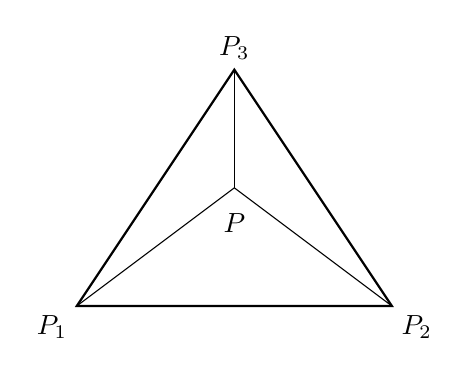
\begin{tikzpicture}
        \draw[thick] (0,0) -- (4,0) -- (2,3) -- cycle;
        \node at (0,0) [below left] {$P_1$};
        \node at (4,0) [below right] {$P_2$};
        \node at (2,3) [above] {$P_3$};
        \node at (2,1.5) [below, yshift=-0.2cm] {$P$};
        \draw (2,1.5) -- (0,0);
        \draw (2,1.5) -- (4,0);
        \draw (2,1.5) -- (2,3);
    \end{tikzpicture}
    \caption{\centering Barycentric coordinates of a point $P$ with respect to a triangle defined by vertices $P_1$, $P_2$, and $P_3$.}
    \label{fig:barycentric}
\end{figure}

Once the barycentric coordinates of a point $P$ are calculated, we can use them to interpolate any value defined at the vertices of the triangle. Given the values $f_1$, $f_2$, and $f_3$ at the vertices $P_1$, $P_2$, and $P_3$ respectively, the interpolated value at point $P$ with barycentric coordinates $\lambda_1$, $\lambda_2$, and $\lambda_3$ is given by:
\[f(P) = \lambda_1 f_1 + \lambda_2 f_2 + \lambda_3 f_3\]

Two things should be noted about barycentric interpolation:
\begin{itemize}
    \item It also interpolates the $x$ and $y$ coordinates of the point $P$ in the triangle. These two conditions and the fact that $\lambda_1 + \lambda_2 + \lambda_3 = 1$ are sufficient to determine the barycentric coordinates of any point in the triangle.
    \item It can be proven that this interpolation is linear; and given that there is a unique linear interpolation for any set of values at the vertices of the triangle, it can be concluded that barycentric interpolation is just another way of performing linear interpolation.
\end{itemize}

\subsection{Ray-triangle intersection}

Any point $P$ in a triangle defined by vertices $P_1$, $P_2$, and $P_3$ can be expressed as a linear combination of the vertices:
\[P = \lambda_1 P_1 + \lambda_2 P_2 + \lambda_3 P_3\]
where $\lambda_1$, $\lambda_2$, and $\lambda_3$ are the barycentric coordinates of $P$ with respect to the triangle. In addition, any point $P'$ on a ray defined by an origin $P_S$ and a direction $\vec{D}$ can be expressed as:
\[P' = P_S + t \vec{D}\qquad t\in \bb{R}^+_0\]

Therefore, determining the intersection point of a ray with a triangle is equivalent to finding the values of $\lambda_1$, $\lambda_2$, $\lambda_3$, and $t$ that satisfy the following system of equations:
\[\begin{cases}
\lambda_1 P_1 + \lambda_2 P_2 + \lambda_3 P_3 = P_S + t \vec{D} \\
\lambda_1 + \lambda_2 + \lambda_3 = 1
\end{cases}\]

It should be noted that the first equation represents three equations, one for each coordinate. Therefore, we have a system of four equations with four unknowns. That system can be fastly solved using Cramer's rule and the triple product of vectors to calculate the determinants. After solving this system, we have to check if the solution is valid:
\begin{itemize}
    \item $t\in \bb{R}^+_0$, as we are only interested in the intersection points that are in the direction of the ray (not behind the ray origin).
    \item $\lambda_i \geq 0$ for $i = 1, 2, 3$, as we are only interested in the intersection points that are inside the triangle (not in the whole plane defined by the triangle).
\end{itemize}

% // TODO: How to solve the system of equations using Cramer's rule and the triple product of vectors to calculate the determinants.



\section{Fewer ray-object intersections}